% XCircuit output "lms7_tdd.tex" for LaTeX input from lms7_tdd.ps
\def\putbox#1#2#3#4{\makebox[0in][l]{\makebox[#1][l]{}\raisebox{\baselineskip}[0in][0in]{\raisebox{#2}[0in][0in]{\scalebox{#3}{#4}}}}}
\def\rightbox#1{\makebox[0in][r]{#1}}
\def\centbox#1{\makebox[0in]{#1}}
\def\topbox#1{\raisebox{-0.60\baselineskip}[0in][0in]{#1}}
\def\midbox#1{\raisebox{-0.20\baselineskip}[0in][0in]{#1}}
   \scalebox{1}{
   \normalsize
   \parbox{6.19792in}{
   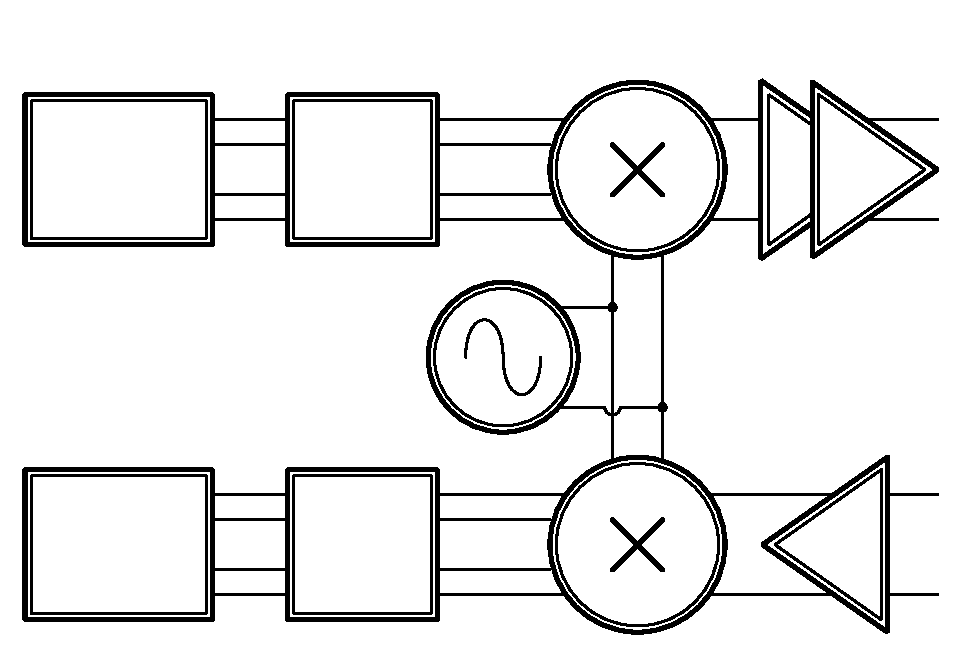
\includegraphics[scale=1]{lms7_tdd}\\
   % translate x=992 y=378 scale 0.38
   \putbox{5.47in}{4.02in}{2.40}{\centbox{\midbox{TX PAD}}}%
   \putbox{5.47in}{1.52in}{2.40}{\centbox{\midbox{LNA}}}%
   \putbox{2.31in}{3.19in}{2.40}{\centbox{\midbox{DAC}}}%
   \putbox{0.70in}{3.19in}{2.40}{\centbox{\midbox{TxTSP}}}%
   \putbox{3.14in}{3.69in}{2.40}{\centbox{\midbox{I}}}%
   \putbox{3.14in}{2.69in}{2.40}{\centbox{\midbox{Q}}}%
   \putbox{1.56in}{3.69in}{2.40}{\centbox{\midbox{I}}}%
   \putbox{1.56in}{2.69in}{2.40}{\centbox{\midbox{Q}}}%
   \putbox{2.31in}{0.69in}{2.40}{\centbox{\midbox{ADC}}}%
   \putbox{0.70in}{0.69in}{2.40}{\centbox{\midbox{RxTSP}}}%
   \putbox{3.14in}{1.19in}{2.40}{\centbox{\midbox{I}}}%
   \putbox{3.14in}{0.19in}{2.40}{\centbox{\midbox{Q}}}%
   \putbox{1.56in}{1.19in}{2.40}{\centbox{\midbox{I}}}%
   \putbox{1.56in}{0.19in}{2.40}{\centbox{\midbox{Q}}}%
   \putbox{2.70in}{1.96in}{2.40}{\rightbox{\midbox{Tx PLL}}}%
   } % close 'parbox'
   } % close 'scalebox'
   \vspace{-\baselineskip} % this is not necessary, but looks better
